\subsection{Crankshaft Position Sensor}
	
	A Crankshaft Position Sensor is shown in Figure \ref{fig-ckpReal}.

	\begin{figure}[htbp]
		\centering
			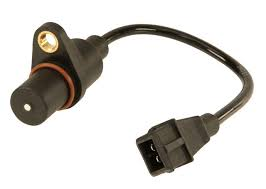
\includegraphics[scale=0.8]{figuras/fig-ckp-real.jpg}
		\caption{\textit{Crankshaft Position Sensor} \cite{ckp-gm}}
		\label{fig-ckpReal}
	\end{figure}

	This sensor is widely used in the automotive industry to determine the speed (RPM) of cranks and gears in the engine. There are several types of CKP sensors, the most common are the variable reluctance type because they have low cost and good accuracy \cite{schroeder2002crankshaft}.
	\par
	Variable reluctance sensors, commonly known as magnetic sensors, are passive sensors, that is, they do not require power for their operation. As the gear in question rotates each tooth of the gear aligns with the sensor, a magnetic flux in the sensor coil changes as the air gap between the sensor and the gear changes. This change in the magnetic field generates induces a voltage pulse at the sensor output. This type of sensors have an analog voltage output where amplitude and frequency vary proportionally to the speed of rotation of a gear. With this type of sensor it is possible to extract data of linear velocity, angular velocity and angular position. However, only the angular velocity data (frequency) is important for this project.

	\begin{figure}[htbp]
		\centering
			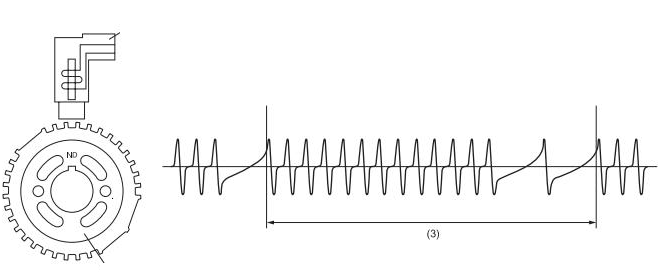
\includegraphics[scale=0.6]{figuras/fig-ckp-signal.png}
		\caption{Magnetic Sensor Signal \cite{cam-sensor-signal}}
		\label{fig-ckpSignal}
	\end{figure}
